\section{Introduction}
\label{sec:intro}

\subsection{Motivation and the failure that defined the question}

Ant scans can turn specimens that are difficult to measure repeatedly into a
source of comparable three-dimensional traits. If every scan is registered to a
common parametric model, quantities such as head width, Weber's length or
appendage proportions can be extracted systematically instead of by hand under
a microscope, which opens a route to studying morphological diversity at
population scale; recent work on \emph{Atta} workers already shows that a 3D
shape space can reveal structure that size scaling alone does not~\cite{imirzian}.
Real scans, however, whether from scAnt photogrammetry~\cite{scant} or
micro-CT, are far from ideal inputs: they contain holes, self-intersections,
arbitrary orientation and missing surface exactly at the thin structures of
greatest anatomical interest (Figure~\ref{fig:raw-scans}).

\begin{figure}[!htb]
\centering
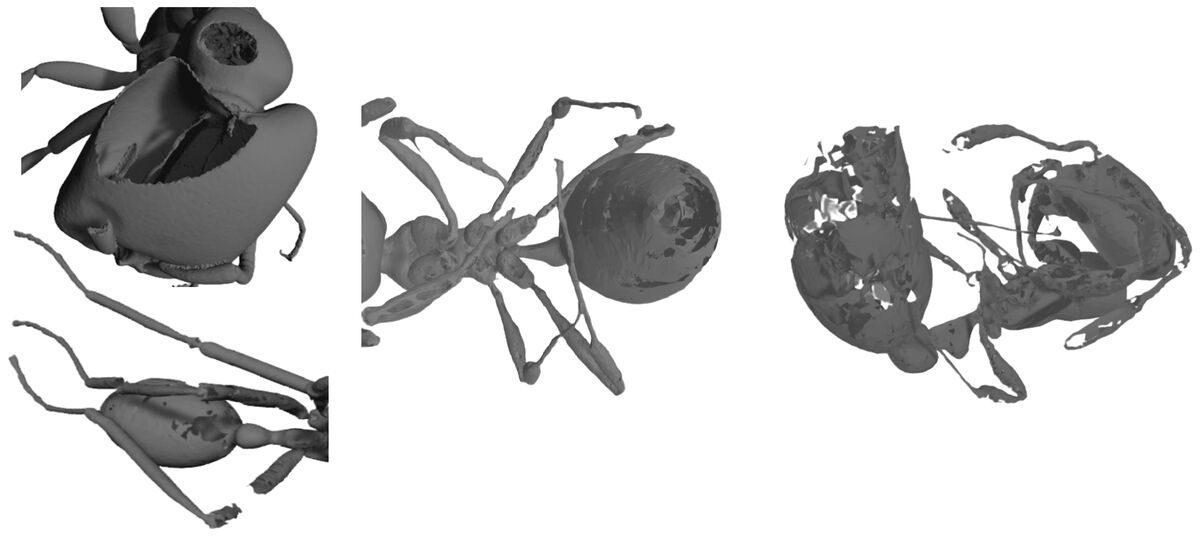
\includegraphics[width=0.50\linewidth]{figures/fig_before_registration.jpg}
\caption[Raw scans before registration]{Raw scans before registration: holes,
self-intersections and missing surface at the structures of greatest
anatomical interest.}
\label{fig:raw-scans}
\end{figure}

In the first week of July 2026, ten preprocessed ant scans were passed through
the registration pipeline. All ten optimisations converged cleanly: the loss
curves showed no divergence and the objective decreased as expected. Four of
the resulting models were nevertheless not recognisable as anatomically
meaningful ants. Legs had collapsed into the gaster and, in some fits, the head
had been absorbed into the thorax. More troublingly, several of these wrong
fits reached a \emph{lower} loss than the runs that had visibly succeeded. The
optimiser had succeeded; the registration had failed. The objective is a
symmetric point-to-point distance between two surfaces: it measures whether the
fitted mesh \emph{covers} the target, not whether vertex $i$ of the template has
landed on the anatomical point it is defined to represent. When the two
diverge, nothing in the pipeline's own numerical output signals it. This
discrepancy is the starting point of the work.

\subsection{Problem formulation: recovering a latent anatomical explanation}
\label{sec:problem}

SMILify~\cite{smilify} extends the optimisation-based SMALify
procedure~\cite{smalify} for the SMAL quadruped model~\cite{smal} to arbitrary
rigged templates, with SMIL (Skinned Multi-Insect Linear) as its insect
instance. Registration recovers, for a scan $T$, the latent variables of a
parametric mesh $M$: shape $\bm\beta$, articulated pose $\bm\theta$, scale $s$
and residual per-vertex deformation $\mathbf d$,
\begin{equation}
(\hat{\bm\beta},\hat{\bm\theta},\hat s,\hat{\mathbf d})
 =\arg\min_{\bm\beta,\bm\theta,s,\mathbf d}\;
 \mathcal{L}\big(M(\bm\beta,\bm\theta,s,\mathbf d),\,T\big).
\label{eq:registration}
\end{equation}
The scan is only a set of surface samples. It carries no vertex identities, no
joint locations and no anatomical labels, yet these are exactly the quantities
the registration is meant to deliver. Anatomical correspondence is therefore an
intended \emph{consequence} of the recovered parameters, not something the
objective observes. Because Equation~\eqref{eq:registration} is non-convex and
its objective sees surfaces only, several different latent configurations can
generate nearly the same surface, and the mapping from observed surface to
anatomical state is not guaranteed to be identifiable.

This is the idea around which the report is organised. The hard part is not
optimising a mesh to a scan; it is recovering the \emph{correct} articulated
explanation from an observation that does not contain anatomical identity.
Every investigation below interrogates that one problem
(Figure~\ref{fig:map}): whether the observation is good enough, whether the
search can reach the right explanation, what additional information would
disambiguate it, how much freedom lets a wrong explanation hide, and whether an
independent reference confirms the result.

\begin{figure}[!htb]
\centering
\begin{tikzpicture}[every node/.style={font=\small},
 n/.style={draw,rounded corners=2pt,minimum height=8mm,align=center,fill=white,inner sep=3pt},
 q/.style={font=\footnotesize\itshape,align=center,text width=3.6cm},
 arr/.style={-{Stealth[length=2mm]}}]
\node[n,fill=gray!12] (o) {Observation\\scan surface $T$};
\node[n,right=2.6cm of o] (l) {Latent explanation\\$\bm\beta,\bm\theta,s,\mathbf d$};
\node[n,right=2.6cm of l,fill=blue!10] (a) {Anatomical identity\\(latent; not directly\\observed)};
\draw[arr](o)--(l); \draw[arr](l)--(a);
\node[q,below=4mm of o] {Is the observation sufficient?\\mesh conditioning};
\node[q,below=4mm of l] {Can the search reach the right explanation, and is it unique?\\initialisation, sampling, robust optimisation, deformation freedom};
\node[q,below=4mm of a] {What would disambiguate it, and how is it verified?\\anatomical priors, correspondence, joint supervision, expert reference};
\end{tikzpicture}
\caption[One inverse problem, several investigations]{The report treats
registration as one inverse problem. Each investigation interrogates a
different link between the observed surface, the recovered parameters and the
anatomical identity that is only indirectly constrained.}
\label{fig:map}
\end{figure}

\subsection{Research questions and technical contributions}

Four research questions make the problem precise:
\begin{enumerate}[label=\textbf{RQ\arabic*.}]
\item Is input mesh quality the dominant limit on registration accuracy?
\item Does a good surface fit imply a correct anatomical fit?
\item Which component (initialisation, sampling, deformation freedom,
correspondence or the objective) limits anatomical recovery, and where along
the body?
\item When a parameter is recovered, when is it a valid biological
measurement?
\end{enumerate}
The internship brief listed six assignments (unify the preprocessing pipeline,
stabilise a Shape-Diameter-Function-based segmentation, integrate neural
initialisation, design a hybrid registration framework, benchmark the result,
document it) that together implied a hypothesis, namely that input mesh quality
is the limiting factor. A controlled test of that hypothesis was negative
(Section~\ref{sec:prep}), and the work was redirected toward RQ2--RQ4.

This work extends the registration pipeline at several levels, from mesh
preparation and anatomical priors to learned initialisation, correspondence and
optimisation, and introduces the experimental machinery required to determine
which of these mechanisms actually preserve anatomical information
(Table~\ref{tab:contrib}). Its contribution has two layers. The
\emph{algorithmic and systems extensions} comprise defect-aware preprocessing,
chain-aware anatomical assignment, a Shape Diameter Function (SDF) prior, a
PointNet-style pose initialiser, sampling-aware and robust optimisation, learned
within-part correspondence descriptors and a hierarchical fitting schedule. The
\emph{diagnostic and evaluation framework} comprises a synthetic round-trip
benchmark with exact vertex identity, oracle ablations, an
adversarial metric test, a corrected and pre-registered expert Joint Alignment
Benchmark (JAB) and an independent measurement-validity analysis. Together they
establish that surface agreement, anatomical correspondence, parameter recovery
and measurement validity are related but distinct properties.

\begin{table}[!htb]
\centering
\caption{Technical contribution map.}
\label{tab:contrib}
\begin{tabular}{@{}L{0.30\linewidth}L{0.62\linewidth}@{}}
\toprule
\textbf{Layer} & \textbf{Components implemented or extended}\\
\midrule
Representation and geometry & Alpha Wrap / ManifoldPlus preprocessing,
 quadric reduction, chain-aware assignment, Shape Diameter Function prior,
 joint-limit integration\\
Learning & PointNet-style pose initialisation, within-part correspondence
 descriptors, template-embedding head with cycle-consistency filtering\\
Optimisation & Objective analysis, sampling audit, robust optimisation,
 hierarchical and staged fitting schedule\\
Evaluation & Synthetic round-trip benchmark, oracle ablations,
 expert Joint Alignment Benchmark, morphometric validation, HPC pipeline\\
\bottomrule
\end{tabular}
\end{table}

\subsection{Structure of the report}

Section~\ref{sec:context} situates the work. Section~\ref{sec:framework} gives
the technical formulation and experimental methodology. Section~\ref{sec:algo}
reports the algorithmic investigations, and Section~\ref{sec:validity} asks
what the recovered representation supports as a measurement.
Section~\ref{sec:discussion} discusses the results against the literature, and
Section~\ref{sec:conclusion} concludes with a research roadmap.
